\documentclass[12pt]{article}
\usepackage{geometry}
\geometry{a4paper}


\usepackage{color}
\usepackage{hyperref}
\usepackage{amsmath}
\usepackage{amsfonts}
\usepackage{amssymb}
\usepackage{graphicx}
\usepackage{tcolorbox}
\usepackage{listings}
\usepackage{here}
\usepackage{txfonts}
\usepackage{algorithm}
\usepackage{algorithmic}
\usepackage{siunitx}
\usepackage{xcolor}

\lstset {language = c++,
  basicstyle = \ttfamily \scriptsize,
  commentstyle = \textit,
  frame = tRBl,
  framesep = 5pt,
  showstringspaces = false,
  numbers = left,
  stepnumber = 1,
  numberstyle = \tiny,
  tabsize = 2,
  keywordstyle = \bfseries \color{blue},
  stringstyle=\color{magenta},
  commentstyle=\color{red},
  morecomment=[l][\color{red}]{\#}
  showstringspaces=false, % don't mark spaces in strings
}
\newcommand{\bi}[1]{\mathbf{#1}}
\newcommand{\bs}[1]{\boldsymbol{#1}}  % bold for greek characters
\newcommand{\bbR}{\mathbb{R}}

\author{Nobuyuki Umetani}


\title{Finite Element Method: \\Solving Poission's Equation}
\author{Nobuyuki Umetani}

\begin{document}
\maketitle


\begin{figure}[htbp!]
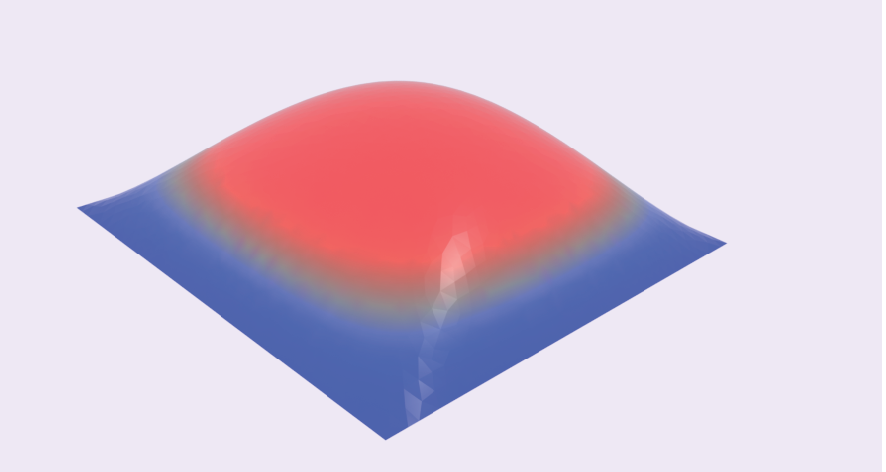
\includegraphics[width=150mm]{images/teaser}
\caption{An example of the Poisson's equation rendered with Blender. }
\end{figure}

\tableofcontents

\section{Weak form of Poisson's Equation}



The Poisson means ``fish" in French, But it's actually It's a mathematician's name who found this equation.

We define a problem to solve Poisson's Equation as:

\begin{tcolorbox}[title=problem setting]
\begin{eqnarray}
\left\{
\begin{array}{rlll}
\nabla^2 \phi &=& f \qquad & ( \quad in \quad V \quad ) \\
\phi               &=& g_1 \qquad & (\quad on \quad S_1 \quad) \\
\frac{\partial \phi}{\partial n } &=& g_2 \qquad & (\quad on \quad S_2 \quad)
\end{array}
\right.
\end{eqnarray}
\end{tcolorbox}

%
There $\phi$ is a scalar field.
%
The scalar field means that there is a scalar value for every point inside this domain.
%
The squared nabla $\nabla^2\phi$ here is actually a divergence of the gradient $\nabla\cdot (\nabla \phi)$.
%
This second order derivative is called Laplacian and you can also write it as $\Delta \phi$. 
%
The gradient of the scalar field makes a vector field and the divergence of the vector field makes a scalar field. 
%
So this Laplacian takes a scalar field and output a scalar field.



You count think the Laplace operator as an indicator of all how much functional is Convex or concave. 
%
In the one-dimensional problem setting, The Poisson's equation becomes a quadratic function. 
%
If the second second derivative is positive, the quadratic function is convex. 
%
If the second derivative is negative, the function is concave.
%
If the second derivative is zero, the the function is linear.
%
The multi-dimensional case is similar to the one dimensional case. 
%
However, if even if the Laplacian is zero, the function is usually still not linear, because we may have a saddle point. 
%
In the case of Saddle Point the second derivative is positive in one Direction and the second derivative is negative Another Direction.
%
So if you compute the sum, these negative and positive derivative cancels out and it becomes zero.




\begin{figure}[htbp!]
	\center
    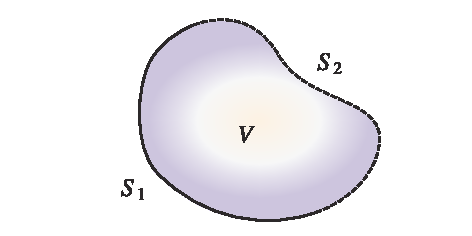
\includegraphics[width=80mm]{images/lap_domain}
    \caption{Problem setting.}
    \label{fig:lap_domain}
\end{figure}

Boundary conditions are classified into two types: Dirichlet condition when the value is determined and Neumann condition when the differential value in the normal direction is determined.
%
These are sometimes called first kind boundary condition, second kind boundary condition, basic boundary condition, natural boundary condition.
If either Dirichlet condition or Neumann condition is not set, the solution is not fixed.
%
Also, the boundary given the Dirichlet condition and the Neumann condition must not overlap.
%
In other words,
%
\begin{eqnarray}
S_1 \cup S_2 = S \qquad S_1 \cap S_2 = \emptyset
\end{eqnarray}




Let's convert the Poission's Equation from the strong form into the weak form
%
Let $\delta\phi$ an arbitraty function that sasisfy
%
\begin{eqnarray}
\delta\phi = 0 \qquad ( \quad on \quad S_1 \quad ).
\end{eqnarray}
%
We multiply $\delta\phi$ into this, and integrate over $V$
%
\begin{eqnarray}
\int_V \nabla^2 \phi \delta \phi dV=\int_V f \delta\phi dV.
\end{eqnarray}


Using the chain rule of the differentiation we have
%
\begin{eqnarray}
\frac{\partial}{\partial x_k}\left(\frac{\partial\phi}{\partial x_k}\delta\phi\right)
=  \frac{\partial}{\partial x_k}\left(\frac{\partial\phi}{\partial x_k}\right)\delta\phi
+ \frac{\partial\phi}{\partial x_k}\frac{\partial\delta\phi}{\partial x_k}
\end{eqnarray}


We integrate this over $V$
%
\begin{eqnarray}
\int_V \nabla \cdot ( \nabla \phi \delta \phi ) dV  =  \int_V \nabla^2 \phi \delta \phi dV  +  \int_V (\nabla \phi) \cdot (\nabla \delta \phi) dV
\end{eqnarray}
%
Substitute the previous expression in the second term. Also, if you exchange the right and left sides,
%
\begin{eqnarray}
\int_V (\nabla \phi) \cdot (\nabla \delta \phi) dV  = \int_V \nabla \cdot ( \nabla \phi \delta \phi ) dV  + \int_V f \delta\phi dV
\end{eqnarray}


Let's take a look at the first term of the right hand side.
%
We apply Gauss's divergence theoremy to this as
%
\begin{eqnarray}
\int_V \nabla \cdot ( \nabla \phi \delta \phi ) dV
&=&  \int_S n \cdot \nabla \phi \delta \phi dS  \\
&=&  \int_S \frac{ \partial \phi }{ \partial n } \delta \phi dS  \\
&=&  \int_{S_1} \frac{ \partial \phi }{ \partial n } \delta \phi dS  +  \int_{S_2} g_2 \delta \phi dS\\
&=&  \int_{S_2} g_2 \delta \phi dS.
\end{eqnarray}

Here we used $\delta \phi=$ on the $S_1$.
%
Substituting this into the above equation yields the Poisson equation written in weak form as follows.

\begin{tcolorbox}[title=Poission equation in Weak Form]
\begin{eqnarray}
\label{eqn:weak_form_poisson}
\left\{ \begin{array}{rlll}
\{\int_V (\nabla \phi) \cdot (\nabla \delta \phi) dV &=& \int_V f \delta\phi dV + \int_{S_2} g_2 \delta \phi dS
& \forall\delta\phi\ni \{ \delta\phi \mid \delta\phi=0 ~(on~S_1) \} \\
\phi &=& g_1
& (\quad on \quad S_1 \quad)
\end{array}\right.
\end{eqnarray}
\end{tcolorbox}




%%%%%%%%%%%%%%%%%%%%%%%%%%%%%
\section{Finite Element Discretization of Weak Form Laplace Equation}

We element - wise write the Laplace equation in the weak form ~ \eqref{eqn: weak_form_poisson}.
%
\begin{eqnarray}
\int_V\frac{\partial\delta\phi}{\partial x_k} \frac{\partial\phi}{\partial x_k}dV  = \int_Vf\delta\phi dV + \int_{S_2} g_2 \delta \phi dS
\end{eqnarray}
%
Then that way.

Here we apply the summary convention for $k$. The above equation is written in integral.
%
Since the integral is sum, it is possible to perform integration while dividing the integral area and add up the integral to calculate the above equation.


Therefore, if you define $ V_e $ and $ S_2 $ as the element divided area as $ {S _ 2} _ e $, the formula can be written as follows.
%
\begin{eqnarray}
\sum_e^{nV_e}\int_{V_e}\frac{\partial\delta\phi}{\partial x_k} \frac{\partial\phi}{\partial x_k}dV
= \sum_e^{nV_e}\int_{V_e}f\delta\phi dV + \sum_e^{{nS_2}_e}\int_{{S_2}_e} g_2 \delta \phi dS
\end{eqnarray}
%

However, $nV_e $, $ {nS_2}_e$ are the number of element divisions of $ V $ and ${S_2}_e$, respectively.

In $ V_e $, it is assumed that functions $ \phi, \delta \phi $ are discretized by the following shape function $ N $. ~
However, in the node $ \bar{n} $ on the surface $ S_1 $ where the fixed boundary condition is set $ \phi^{\bar{n}} = g_1 $, $ \delta \phi^{\bar{n}}=0$.

\begin{eqnarray}
\phi &=& N^n\phi^n\\
\delta\phi &=& N^m\delta\phi^m
\end{eqnarray}


Likewise, within $ {S _ 2} _ e $, functions $ \ phi, \ delta \ phi $ are discretized by the following shape function $ \ bar {N} $.

\begin{eqnarray}
\phi &=& \bar{N}^n\phi^n\\
\delta\phi &=& \bar{N}^m\delta\phi^m
\end{eqnarray}


Substitute $\phi,\delta\phi$ interpolated by shape function into the above equation

\begin{eqnarray}
\sum_{e}^{nV_e}\int_{V_e}\frac{\partial N^m}{\partial x_k}\frac{\partial N^n}{\partial x_k}\phi^n \delta\phi^m dV_e
= \sum_{e}^{nV_e}\int_{V_e} f N^m \delta\phi^m dV + \sum_{e}^{{nS_2}_e}\int_{{S_2}_e} g_2 \bar{N}^m \delta\phi^m dS
\end{eqnarray}


Here, $\phi^n, \delta \phi^m$ is put out of the integral. They are summarized as follows.

\begin{eqnarray}
\delta\phi^m  \left(  \sum_{e}^{nV_e}\int_{V_e}\frac{\partial N^m}{\partial x_k}\frac{\partial N^n}{\partial x_k}dV  \right) \phi^n   =  \delta\phi^m  \left(  \sum_{e}^{nV_e}\int_{V_e} f N^m  dV  +  \sum_{e}^{{nS_2}_e}\int_{S_2} g_2 \bar{N}^m  dS  \right)
\end{eqnarray}


These can be written in the matrix form as:
%
\begin{tcolorbox}[title=discretized poission equation in weak form]
\begin{eqnarray}
\delta\phi^mA^{m,n}\phi^n &=& \delta\phi^mb^m\\
A^{m,n} &=& \sum_{e}^{nV_e}A_e^{a,b}
\end{eqnarray}
 (here elemental node number $a$,$b$ corresponds to global node number $m$,$n$)
\end{tcolorbox}

\begin{tcolorbox}[title=element-wise stiffness matrix]
\begin{eqnarray}
A_e^{a,b} &=& \int_{V_e}\frac{\partial N^a}{\partial x_k}\frac{\partial N^b}{\partial x_k}dV\\
b^{m} &=& \sum_{e}^{nV_e}\int_{V_e} f N^m  dV + \sum_{e}^{{nS_2}_e}\int_{S_2} g_2 \bar{N}^m  dS
 \end{eqnarray}
\end{tcolorbox}

The matrix expression of the above equation is as follows. $\delta\bi{\phi}^T\bi{A}\bi{\phi}=\delta\bi{\phi}^T\bi{b}$


%%%%%%%%%%%%%%%%%%%%%%%%%%%
\subsection{Treatment of Boundary Condition}

As it is, it can not be solved as a simultaneous linear equation. ~
On node $\bar{n}$ on fixed side boundary condition $S_1$ $\phi^{\bar{n}}=g_1$, $\delta\phi^{\bar{n}}=0$ was Given. Let the value of $\phi$ on the surface $S_1$ be $\bar{\phi}$.
Also, if the values ​​of $\phi$, $\delta\phi$ at points other than on the unknown surface $S_1$ are $\hat{\phi}$, $\delta\hat{\phi}$, the above equation becomes as follows.

\begin{eqnarray}
\left(\begin{array}{cc}
\delta\hat{\phi} & 0
\end{array}\right)
\bi{A}
\left(\begin{array}{c}
\hat{\phi}\\ \bar{\phi}
\end{array}\right)
 =
\left(\begin{array}{cc}
\delta\hat{\phi} & 0
\end{array}\right)\bi{b}
\end{eqnarray}


Thanks can be expanded as:
%
\begin{eqnarray}
\delta\hat{\phi}\hat{\bi{A}}\hat{\phi}=\delta\hat{\phi}\left(\hat{\bi{b}}-\tilde{\bi{A}}\bar{\phi}\right)
\end{eqnarray}



Here $\hat{\bi{A}}$ is the matrix taken out from $\bi{A}$ for the unknown elements.
%
$\tilde{\bi{A}}$ is the matrix taken out from $\bi{A}$ for elements where column is unknown and row is known.
%
In addition, $\hat{\bi{b}}$ is a vector that has extracted the components of $\bi{b}$ for unknown degrees of freedom.

Note that we had to satisfy the above equation for the value of arbitrary $\hat{\phi}$

\begin{eqnarray}
\hat{\bi{A}}\hat{\phi}=\hat{\bi{b}}-\tilde{\bi{A}}\bar{\phi}
\end{eqnarray}


It can be written as By adopting this form, it is possible to calculate and solve the solution.



Solving the residuals and increments gives a simpler formula. Let's solve the above expression for increment.
Substituting $\hat{\phi}=\hat{\phi}_0+\Delta\hat{\phi}$

\begin{eqnarray}
\hat{\bi{A}}(\hat{\phi}_0+\Delta\hat{\phi})=\hat{\bi{b}}-\tilde{\bi{A}}\bar{\phi}
\end{eqnarray}



When this is modified,

\begin{eqnarray}
\hat{\bi{A}}\Delta\hat{\phi}=\hat{\bi{b}}-\tilde{\bi{A}}\bar{\phi} - \hat{\bi{A}}\hat{\phi}_0=\hat{\bi{r}}_0
\end{eqnarray}



However, $\hat{\bi{r}}_0$ only sets the unknown degrees of freedom of the residuals $\bi{r}_0=\bi{b} - \bi{A}\bi{\phi}_0$ It was taken out.
%
Calculating $\bi{A}\bi{\phi}_0$ may be more computation-intensive than computing $ \tilde{A}\bar{\phi}$.
%
However, when solving a nonlinear equation, since it is solved for the residuals and increments, the residuals have to be computed in any way, which does not become extra labor.
%
We often use this type of boundary condition processing when solving nonlinear equations.

%%%%%%%%%%%%%%%%%
\section{Element-wise Discretization}

In the case of a simple shape, integration can be performed analytically without using numerical integration. This case is briefly summarized.

\subsection{simplex (triangle, tetrahedron) primary element}

The primary interpolation function of triangles and tetrahedrons is linear. Write the interpolation function for node $a$ like $L^a$.

Spatial differentiation is constant as it is linear. That is, $\frac{\partial L^a}{\partial x^i}$ is constant within the element. Since the integrand in determining the stiffness matrix is ​​also a constant, we can perform integration by multiplying this constant by the area or volume of the element. By using this we can write an element stiffness matrix as follows.

\begin{eqnarray}
A_e^{a,b}=\int_{V_e}\frac{\partial N^a}{\partial x_k}\frac{\partial N^b}{\partial x_k}dV=\Delta\frac{\partial L^a}{\partial x_k}\frac{\partial L^b}{\partial x_k}
\end{eqnarray}


However, $\Delta$ is the area of ​​a triangle in the case of two dimensions, and the volume of tetrahedrons in the case of three dimensions.


here,

\begin {itemize}
\item area = $\Delta$,
\item dldx[a][i] = $\partial L^a / \partial x_i$
\item emat[a][b] = $A_e^{a,b}$
\end {itemize}

In the case where variables correspond to each other,
An example of the program is as follows


\begin {lstlisting}[frame=single, caption=C++ code to compute an element stiffness matrix]
for(int inoel=0; inoel<nnoel; ++inoel){
for(int jnoel=0; jnoel<nnoel; ++jnoel){
  double dtmp1 = 0.0;
  for(int idim=0; idim<ndim; ++idim){
    dtmp1+=dldx[inoel][idim]*dldx[jnoel][idim];
  }
  emat[inoel][jnoel]=area*dtmp1;
}
}
\end{lstlisting}

\subsection{Orthogonal Quadrilateral Element}

\begin{eqnarray}
\left\{\begin{array}{l}
N^1=(1-\frac{x}{h_x})(1-\frac{y}{h_y})\\
N^2=\frac{x}{h_x}(1-\frac{y}{h_y})\\
N^3=\frac{x}{h_x}\frac{y}{h_y}\\
N^4=(1-\frac{x}{h_x})\frac{y}{h_y}
\end{array}\right.
\end{eqnarray}


When calculating these x derivatives and y derivatives,

\begin{eqnarray}
\left\{\begin{array}{ll}
\frac{\partial N^1}{\partial x}=-\frac{1}{h_x}(1-\frac{y}{h_y})   &   \frac{\partial N^1}{\partial y}=-(1-\frac{x}{h_x})\frac{1}{h_y}\\      \frac{\partial N^2}{\partial x}=\frac{1}{h_x}(1-\frac{y}{h_y})   &   \frac{\partial N^2}{\partial y}=-\frac{x}{h_x}\frac{1}{h_y}\\
\frac{\partial N^3}{\partial x}=\frac{1}{h_x}\frac{y}{h_y}   &   \frac{\partial N^3}{\partial y}=\frac{x}{h_x}\frac{1}{h_y}\\
\frac{\partial N^4}{\partial x}=-\frac{1}{h_x}\frac{y}{h_y}   &   \frac{\partial N^4}{\partial y}=(1-\frac{x}{h_x})\frac{1}{h_y}
\end{array}\right.
\end{eqnarray}


When integrating, it is as follows,

\begin{align}
\int_{V_e}\frac{\partial N^1}{\partial x}\frac{\partial N^1}{\partial x}dV
&= \int_{V_e}\frac{\partial N^2}{\partial x}\frac{\partial N^2}{\partial x}dV
= \int_{V_e}\frac{\partial N^3}{\partial x}\frac{\partial N^3}{\partial x}dV
= \int_{V_e}\frac{\partial N^4}{\partial x}\frac{\partial N^4}{\partial x}dV
= \frac{1}{3}\frac{h_y}{h_x}\\
\int_{V_e}\frac{\partial N^1}{\partial x}\frac{\partial N^2}{\partial x}dV
&= \int_{V_e}\frac{\partial N^3}{\partial x}\frac{\partial N^4}{\partial x}dV
= -\frac{1}{3}\frac{h_y}{h_x}\\
\int_{V_e}\frac{\partial N^1}{\partial x}\frac{\partial N^3}{\partial x}dV
&= \int_{V_e}\frac{\partial N^2}{\partial x}\frac{\partial N^4}{\partial x}dV
= -\frac{1}{6}\frac{h_y}{h_x}\\
\int_{V_e}\frac{\partial N^1}{\partial x}\frac{\partial N^4}{\partial x}dV
&= \int_{V_e}\frac{\partial N^2}{\partial x}\frac{\partial N^3}{\partial x}dV
= +\frac{1}{6}\frac{h_y}{h_x}
\end{align}



\begin{align}
\int_{V_e}\frac{\partial N^1}{\partial y}\frac{\partial N^1}{\partial y}dV
&= \int_{V_e}\frac{\partial N^2}{\partial y}\frac{\partial N^2}{\partial y}dV
= \int_{V_e}\frac{\partial N^3}{\partial y}\frac{\partial N^3}{\partial y}dV
= \int_{V_e}\frac{\partial N^4}{\partial y}\frac{\partial N^4}{\partial y}dV
= \frac{1}{3}\frac{h_x}{h_y}\\
\int_{V_e}\frac{\partial N^1}{\partial y}\frac{\partial N^2}{\partial y}dV
&= \int_{V_e}\frac{\partial N^3}{\partial y}\frac{\partial N^4}{\partial y}dV
= \frac{1}{6}\frac{h_x}{h_y}\\
\int_{V_e}\frac{\partial N^1}{\partial y}\frac{\partial N^3}{\partial y}dV
&= \int_{V_e}\frac{\partial N^2}{\partial y}\frac{\partial N^4}{\partial y}dV
= -\frac{1}{6}\frac{h_x}{h_y}\\
\int_{V_e}\frac{\partial N^1}{\partial y}\frac{\partial N^4}{\partial y}dV
&= \int_{V_e}\frac{\partial N^2}{\partial y}\frac{\partial N^3}{\partial y}dV
= -\frac{1}{3}\frac{h_x}{h_y}
\end{align}


Therefore, the element stiffness matrix is ​​as follows

\begin{eqnarray}
A^{a,b}
&=&\int_{V_e}\frac{\partial N^a}{\partial x}\frac{\partial N^b}{\partial x}+\frac{\partial N^a}{\partial y}\frac{\partial N^b}{\partial y}dV \\
&=&\frac{1}{6h_yh_x}\left[\begin{array}{llll}                                         2(h_y^2+h_x^2) & -2h_y^2+h_x^2& -h_y^2-h_x^2 & h_y^2-2h_x^2\\                   -2h_y^2+h_x^2 & 2(h_y^2+h_x^2) & h_y^2-2h_x^2 & -h_y^2-h_x^2\\                  -h_y^2-h_x^2 & h_y^2-2h_x^2 & 2(h_y^2+h_x^2) & -2h_y^2+h_x^2\\                  h_y^2-2h_x^2 & -h_y^2-h_x^2 & -2h_y^2+h_x^2 & 2(h_y^2+h_x^2)\end{array}\right]
\end{eqnarray}



\subsection{Orthogonal Qquare Element}1

Here, when $h_x=h_y$ is specified, it becomes as follows.

\begin{eqnarray}
A^{a,b}=\left[\begin{array}{cccc}\frac{2}{3}&-\frac{1}{6}&-\frac{1}{3}&-\frac{1}{6}\\        -\frac{1}{6}&\frac{2}{3}&-\frac{1}{6}&-\frac{1}{3}\\        -\frac{1}{3}&-\frac{1}{6}&\frac{2}{3}&-\frac{1}{6}\\        -\frac{1}{6}&-\frac{1}{3}&-\frac{1}{6}&\frac{2}{3}\\ \end{array}\right]
\end{eqnarray}


Stencils at each point are as follows
%
\begin{eqnarray}
\frac{1}{3}\left[\begin{array}{ccc}-1&-1&-1\\-1&8&-1\\-1&-1&-1\end{array}\right]
\end{eqnarray}



\section{Examples}

We consider an example of Poisson's equation problem where the domain is a unit square and all the four edges are Dirichlet boundary condition with value zero ($\phi=0$). 
%
We set the source is one ($f=1$).
%
Figure~\ref{fig:example} shows an example.

\begin{figure}[htbp!]
\center
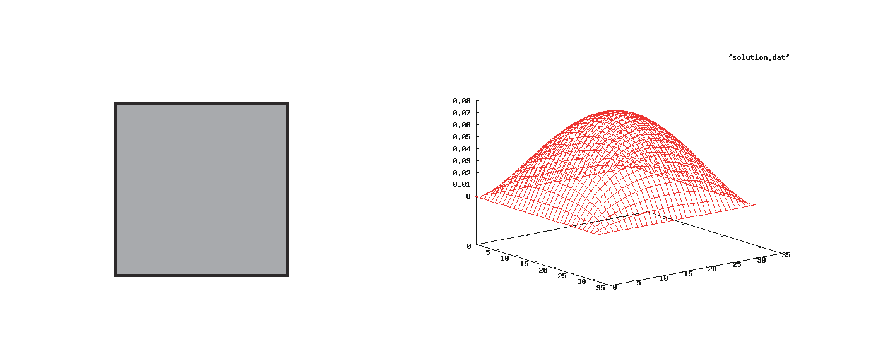
\includegraphics[width=150mm]{images/example}
\caption{Example of the solution of Poisson's equation}
\label{fig:example}
\end{figure}


%%%%%%%%%%%%%%%%%%%%%%%%%%%%%%%%%%%%%%%%%%%%%%%%%%%%%%%%%%%%%%%%%%
\section{Axisymmetric Problem}
Let's consider an axisymmetric problem. 
%
In other words, consider the case where there is no change in the circumferential direction in the analysis region, the boundary conditions and the physical properties. 
%
In this case, the solution of the equation also becomes axisymmetric, and thus it is possible to handle three-dimensional problems two-dimensionally while ignoring the change in the thickness direction.

\begin{figure}[htbp!]
	\center
    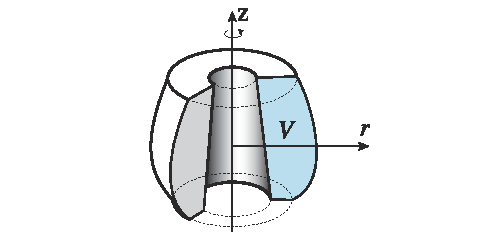
\includegraphics[width=80mm]{images/cylinder_domain}
    \caption{Axisymmetric problem setting}
    \label{fig:cylinder_domain}
\end{figure}


\subsection{Laplace Equation in Cylindrical Coordinates}

When considering the cylindrical coordinate system, the target field is expressed as the distance to the axis and the variable of the z coordinate. 
%
For simplicity, it is assumed that the rotation axis corresponds to the z axis. 
%
At this time, the field is represented as follows.

\begin{eqnarray}
\phi(x,y,z) = \phi(r,z)\;\;\; r=\sqrt{x^2+y^2}
\end{eqnarray}

Calculating these differentiations yields the following.

\begin{equation}
\left\{\begin{array}{l}
\frac{\partial r}{\partial x} = \frac{x}{\sqrt{x^2+y^2}} = \frac{x}{r}  \\
\frac{\partial^2 r}{\partial x^2} = \frac{\partial}{\partial x}(\frac{x}{r}) = \frac{1}{r} - \frac{x^2}{r^3}\\
\frac{\partial r}{\partial y} = \frac{y}{\sqrt{x^2+y^2}}=\frac{y}{r} \\
 \frac{\partial^2 r}{\partial y^2} = \frac{\partial}{\partial y}(\frac{y}{r}) = \frac{1}{r} - \frac{y^2}{r^3}\\
\frac{\partial^2 r}{\partial x\partial y} = -\frac{xy}{r^3}
\end{array} \right.
\end{equation}

Using these

\begin{eqnarray}
\frac{\partial^2 \phi}{\partial x^2}
&=& \frac{\partial}{\partial x}\left(\frac{\partial\phi}{\partial x}\right) \\
&=& \frac{\partial}{\partial x}\left\{\left(\frac{\partial\phi}{\partial r}\right)\left(\frac{\partial r}{\partial x}\right)\right\}  \\
&=& \left(\frac{\partial^2\phi}{\partial r^2}\right)\left(\frac{\partial r}{\partial x}\right)^2 + \left(\frac{\partial\phi}{\partial r}\right)\left(\frac{\partial^2 r}{\partial x^2}\right)\\
&=& \left(\frac{\partial^2\phi}{\partial r^2}\right)\left(\frac{x}{r}\right)^2 + \left(\frac{\partial\phi}{\partial r}\right)\left(\frac{1}{r} - \frac{x^2}{r^3}\right)
\end{eqnarray}


\begin{eqnarray}
\frac{\partial^2 \phi}{\partial y^2} = \left(\frac{\partial^2\phi}{\partial r^2}\right)\left(\frac{y}{r}\right)^2 + \left(\frac{\partial\phi}{\partial r}\right)\left(\frac{1}{r} - \frac{y^2}{r^3}\right)
\end{eqnarray}


By using these, the Laplace operator in orthogonal coordinates is calculated as follows.

\begin{eqnarray}
\left(\frac{\partial^2}{\partial x^2} + \frac{\partial^2}{\partial y^2}+\frac{\partial^2}{\partial z^2}\right)\phi(r,z)
&=&  \left(\frac{\partial^2\phi}{\partial r^2}\right)\left(\frac{x^2+y^2}{r^2}\right) + \left(\frac{\partial\phi}{\partial r}\right)\left(\frac{2}{r} - \frac{x^2+y^2}{r^3}\right) + \frac{\partial^2 \phi}{\partial z^2}\\
&=& \frac{\partial^2\phi}{\partial r^2} + \frac{1}{r}\left(\frac{\partial\phi}{\partial r}\right) + \frac{\partial^2 \phi}{\partial z^2}
\end{eqnarray}


Therefore, the Laplace equation in the cylindrical coordinate system of the axisymmetric problem can be written as follows


\begin{tcolorbox}[title=Laplace's Equation in Cylindrical Coordinate]
\begin{eqnarray}
\frac{\partial^2\phi}{\partial r^2} + \frac{1}{r}\left(\frac{\partial\phi}{\partial r}\right) + \frac{\partial^2 \phi}{\partial z^2} = f(r,z)
\end{eqnarray}
\end{tcolorbox}


$f$ represents the source per unit volume. Note that this $f$ is also axisymmetric.

%%%%%%%%%%%%%%%%%%%%%%%%%%%%%%%%%
\subsection{Weak Formalization}

Let us assume that a fixed boundary condition is defined axially symmetrically and a natural boundary condition is defined.


The above equation is multiplied by the axisymmetric function $\delta\phi(r,z)$ which becomes 0 on the fixed boundary and integrated over the whole area.

\begin{eqnarray}
\int_V\delta\phi (\nabla^2\phi+f) dxdydz = 0\;\; \forall \delta\phi
\end{eqnarray}


\begin{eqnarray}
\left\{\begin{array}{l}
x\rightarrow rsin\theta\\ y\rightarrow rcos\theta\\ z\rightarrow z
\end{array}\right.
\end{eqnarray}



The absolute value of Jacobian in this case is

\begin{eqnarray}
\det J(r,\theta,z)
=
\det \left[\begin{array} {lll}
\sin\theta & r \cos\theta & 0 \\
\cos\theta & -r\sin\theta & 0 \\
0 & 0 &  1
\end{array}\right] = r
\end{eqnarray}

Therefore, it becomes $dxdydz = r drd\theta dz$. When this is substituted above,

\begin{eqnarray}
&& \int_V\delta\phi (\nabla^2\phi+f) r drd\theta dz = 0\;\; \forall \delta\phi\\
&\Leftrightarrow& \int_\theta\int_z\int_r \delta\phi\left(\frac{\partial^2\phi}{\partial r^2} + \frac{1}{r}\left(\frac{\partial\phi}{\partial r}\right) + \frac{\partial^2 \phi}{\partial z^2} + f(r,z)\right) r drdzd\theta = 0
\end{eqnarray}

Here, considering that there is no change in the $\theta$ direction, the integration of $\theta$ can be excluded. We convert this to weak form using Gauss' divergence theorem

\begin{eqnarray}
&& \int_z\int_r \delta\phi\left(\frac{\partial^2\phi}{\partial r^2} + \frac{1}{r}\left(\frac{\partial\phi}{\partial r}\right) + \frac{\partial^2 \phi}{\partial z^2} + f(r,z)\right) r drdz = 0\;\;\forall \delta\phi\\
&\Leftrightarrow&         \int_z\int_r \left(\frac{\partial}{\partial r}\left(\delta\phi r\frac{\partial\phi}{\partial r}\right) - r\frac{\partial\delta\phi}{\partial r}\frac{\partial \phi}{\partial r} + \frac{\partial}{\partial z}\left(\delta\phi r\frac{\partial \phi}{\partial z}\right) - r\frac{\partial\delta\phi}{\partial z}\frac{\partial\phi}{\partial z} + \delta\phi rf(r,z)\right) drdz = 0\;\;\forall \delta\phi\\
&\Leftrightarrow&               \int_z\int_r   r\frac{\partial\delta\phi}{\partial r}\frac{\partial \phi}{\partial r} + r\frac{\partial\delta\phi}{\partial z}\frac{\partial\phi}{\partial z} drdz \\
&& = \int_z\int_r \frac{\partial}{\partial r}\left(\delta\phi r\frac{\partial\phi}{\partial r}\right) + \frac{\partial}{\partial z}\left(\delta\phi r\frac{\partial \phi}{\partial z}\right) + \delta\phi rf(r,z) drdz\;\;\forall \delta\phi\\
&\Leftrightarrow&               \int_z\int_r   r\frac{\partial\delta\phi}{\partial r}\frac{\partial \phi}{\partial r} + r\frac{\partial\delta\phi}{\partial z}\frac{\partial\phi}{\partial z} drdz\\
&& = \int_\Gamma n_r\left(\delta\phi r\frac{\partial\phi}{\partial r}\right) + n_z\left(\delta\phi r\frac{\partial \phi}{\partial z}\right)ds + \int_z\int_r \delta\phi rf(r,z) drdz\;\;\forall \delta\phi\\
&\Leftrightarrow&               \int_z\int_r   r\frac{\partial\delta\phi}{\partial r}\frac{\partial \phi}{\partial r} + r\frac{\partial\delta\phi}{\partial z}\frac{\partial\phi}{\partial z} drdz = \int_\Gamma \delta\phi r\frac{\partial\phi}{\partial n}ds + \int_z\int_r\delta\phi rf(r,z) drdz\;\;\forall \delta\phi\\
\end{eqnarray}

The two-dimensional area of ​​the cross section is $\Omega$, $\frac{\partial \phi}{\partial n}=t$ is as follows.

\begin{tcolorbox}[title=Laplace Equation in Cylindrical Coordinate in Weak Form]
\begin{eqnarray}
\int_\Omega r\frac{\partial\delta\phi}{\partial r}\frac{\partial \phi}{\partial r} + r\frac{\partial\delta\phi}{\partial z}\frac{\partial\phi}{\partial z} drdz = \int_\Gamma \delta\phi t rds + \int_\Omega\delta\phi f(r,z) rdrdz\;\;\forall \delta\phi\\
\end{eqnarray}
\end{tcolorbox}



\subsection{Finite Element Discretization}

In the above weak formalization, the problem of axisymmetry is reduced to a two-dimensional problem of cross section. Let's suppose that the area of ​​the cross section is divided into meshes. The integral is calculated by dividing the integral domain by element unit and adding it, the above equation becomes as follows.

\begin{eqnarray}
\sum_e\int_{\Omega_e} r\frac{\partial\delta\phi}{\partial r}\frac{\partial \phi}{\partial r} + r\frac{\partial\delta\phi}{\partial z}\frac{\partial\phi}{\partial z} drdz = \sum_e\int_{\Gamma_e} \delta\phi trds + \sum_e\int_{\Omega_e}\delta\phi f(r,z) rdrdz\;\;\forall \delta\phi\\
\end{eqnarray}


Given discretization using the Galerkin method, assume that $\delta\phi$ and $\phi$ are elementally divided on the two-dimensional cross section using the interpolation function $N(r,z)$ as follows.

\begin{eqnarray}
\phi = N^n\phi^n,\;\;\;\; \delta\phi = N^m\phi^m
\end{eqnarray}



Suppose the number $m,n$ in the element corresponds to the number $a,b$ in the whole. Also, it is assumed that the elements of the surface on which the natural boundary condition is imposed are discretized by the shape function $\bar{N}$. When this is substituted above, it becomes as follows.

\begin{eqnarray}
&&\sum\int_{\Omega_e} r\frac{\partial N^m\delta\phi^m}{\partial r}\frac{\partial  N^n\phi^n}{\partial r} + r\frac{\partial N^m\delta\phi^m}{\partial z}\frac{\partial N^n\phi^n}{\partial z} drdz \\
 && = \sum_e\int_{\Gamma_e} \bar{N}^m\delta\phi^m trds + \sum_e\int_{\Omega_e} N^m\delta\phi^m f(r,z) rdrdz\;\;\forall \delta\phi\\
&\Leftrightarrow&  \sum_e\left[\delta\phi^m\int_\Omega r\frac{\partial N^m}{\partial r}\frac{\partial  N^n}{\partial r} + r\frac{\partial N^m}{\partial z}\frac{\partial N^n}{\partial z} drdz\phi^n \right] \\
&& = \sum_e\left[\delta\phi^m \int_{\Gamma_e} \bar{N}^mtrds\right] + \sum_e\left[\delta\phi^m\int_{\Omega_e} N^m f(r,z) rdrdz\right]\;\;\forall \delta\phi\\
&\Leftrightarrow&  \sum_e\left[\delta\phi^m A_e^{mn}\phi^n \right] = \sum_e\left[\delta\phi^m {f_e}_{out}^m\right] + \sum_e\left[\delta\phi^m{f_e}_{in}^m\right]\;\;\forall \delta\phi\\
&\Leftrightarrow&  \delta\phi^a\left[ \sum_e A_e^{mn} \right]\phi^b = \delta\phi^a\left[ \sum_e {f_e}_{out}^m\right] + \delta\phi^a\left[ \sum_e {f_e}_{in}^m\right]\;\;\forall \delta\phi\\
&\Leftrightarrow&  \delta\phi^aA^{ab}\phi^b = \delta\phi^a f_{out}^a + \delta\phi^a f_{in}^a\;\;\forall \delta\phi
\end{eqnarray}


However, $A_e^{mn}$ is an element stiffness matrix, ${f_e}^m$ is an external force vector and can be written as follows.

\begin{tcolorbox}[title=element wise stiffness matrix]
\begin{eqnarray}
A_e^{mn}=\int_\Omega r\frac{\partial N^m}{\partial r}\frac{\partial  N^n}{\partial r} + r\frac{\partial N^m}{\partial z}\frac{\partial N^n}{\partial z} drdz
\end{eqnarray}
\end{tcolorbox}

\begin{tcolorbox}[title=external force]
\begin{eqnarray}
{f_e}_{out}^m &=& \int_{\Gamma_e} \bar{N}^m\delta\phi^m trds\\
{f_e}_{in}^m &=& \int_{\Omega_e} N^m\delta\phi^m f(r,z) rdrdz
\end{eqnarray}
\end{tcolorbox}


\subsection{Element Stiffness Matrix in Triangle Primary Element (Linear Element)}

In simple cases like triangular primary elements, we can integrate element stiffness matrices analytically. A linear interpolation function with such a primary element is expressed by using $L$ instead of $N$.

Since the distance $r$ to the axis changes primarily in the triangle

\begin{eqnarray}
r = L^p r^p
\end{eqnarray}

Thus, it can be obtained by interpolating the value of the node.

\begin{eqnarray}
A_e^{mn}
&=&\int_\Omega L^pr^p\frac{\partial L^m}{\partial r}\frac{\partial  L^n}{\partial r} + L^pr^p\frac{\partial L^m}{\partial z}\frac{\partial L^n}{\partial z} drdz\\
&=& \frac{1}{3}(r^1+r^2+r^3)\left\{\frac{\partial L^m}{\partial r}\frac{\partial  L^n}{\partial r} + \frac{\partial L^m}{\partial z}\frac{\partial L^n}{\partial z} \right\}\Delta
\end{eqnarray}


However, $\Delta$ is the area of ​​a triangle. In the end, in this case, it turns out that the distance at the position of the center of gravity is multiplied by the element rigidity of the Laplace equation of the two-dimensional triangle.


%%%%%%%%%%%%%%%%%%%%%%%%%
\end{document}
